\section{Genome sequencing}

\subsection{Sanger sequencing}

\paragraph*{Introduction}
The ``Sanger method'' for DNA sequencing was developed in 1977 by  Frederick
Sanger (1918-2013).
Since then the method had many improvements.
Around 1990 the original radioactive labelling was replaced by fluorescent
dyes and the first automatic DNA sequencers appeared. 
They were called automatic because they could output the actual DNA sequence.

The automatic Sanger DNA sequencers can produce 96 ``reads'' per run. 
The length of each read can be up to 1000 bases long, but the quality
deteriorates  progressively.


\paragraph*{Fragment separation}

The strategy is based on the possibility to create a lot of subfragments of
the region to be sequenced.

1) All fragments must start at the same position 

2) The termination of the fragments should be according to 4 different
classes (A,C,T,G)

This can be done by synthesis, using DNA polymerases. 
The DNA to be sequenced must be present in many copies. 
The DNA polymerases will start all the subfragments from a specific primer
that will define the unique start common to all subfragments.


\paragraph*{Locus sequencing}

If we want to sequence a specific genomic locus (for instance a human
locus that is suspected to carry a mutation) then we can amplify it
by PCR.

After 30-35 cycles of PCR, many millions DNA fragments will be amplified
and will be ready for sequencing. \\

\textbf{Definition of locus}: A locus (plural loci) in genetics is the position
of a gene on a chromosome.
Each chromosome carries many genes; humans' estimated ``haploid'' protein
coding genes are 19,000-20,000, on the 23 different chromosomes.

A variant of the similar DNA sequence located at a given locus is called
an allele. \\

Some genomic loci are variable in the population.
For instance a locus could be found in 60\% of the individuals as a C and
in 40\% as a T.
There are several millions such loci in the human population, about 1/500
bases.
If a variant is present in at least 1\% of the population is called
\textbf{polymorphism}, otherwise is it is called \textbf{mutation}. 

We should also remember that we are diploid.
So we have two copies of each gene, one from each parent.

Polymorphic loci are commonly used to correlate DNA samples,
even very small amount that can be amplified by PCR.
They can also be used to establish paternity and other genetic
relationships.
A few tens of highly polymorphic SNP's (single nucleotide polymorphisms)
can be used, alternatively other kinds of polymiorphisms can be used,
such as short tandem repeats.

\subsection{The problem of whole genome sequencing}

\paragraph*{Problems}
\begin{itemize}
	\item Genomes are large from million to billion bases long
	\item DNA sequences produced by Sanger sequencing are typically 500-1000
bases long; the sequences produced by sequencers are called reads.
They are not enough.
\end{itemize}

\paragraph*{Possible strategies}
\begin{itemize}
	\item Use genetic engineering to produce contiguous fragments of DNA,
then sequence each fragment, knowing where in advance it is positioned
(this approach is unfeasible)
	\item Use a \textbf{shotgun approach}, that is the sequencing of random
genomic fragments, then analyzed by suitable computer program to re-assemble
the genome.
\end{itemize}

... the only alternative seems to be the shotgun approach

\subsection{Shotgun}

Sometimes, hierarchical shotgun assembly may be a good compromise. 
BACs (Bacterial Artificial Chromosomes) are DNA vectors used in molecular
biology.

A \textbf{vector} is a DNA molecule used as a vehicle to artificially
carry foreign genetic material into another cell, where it can be replicated
and/or expressed. 

They can host up to 150 kbp of DNA. 
When transfected into E. coli they replicate as a chromosome thus allowing
the preparation of that particular piece of DNA.
The genome is cloned into a BAC library, with genomic inserts of 100-150 Kbases,
then BAC clones are sequenced independently using the shotgun approach.
The BAC clones can be randomly chosen, or can be selected for minimal overlap.
The assembly process is simplified, but a lot of work is required for the production of the BAC library.
Even more work would be required for the selection of BACs with minimal overlapping.

\begin{figure}[H]
  \centering
  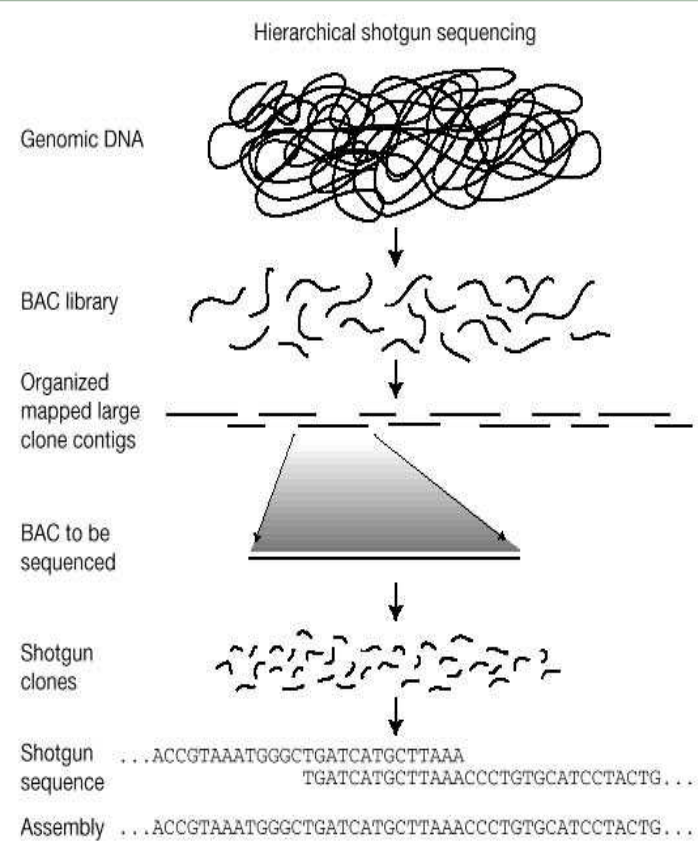
\includegraphics[scale=0.4]{shotgun}
  \caption{shotgun steps}
  \label{fig:shotgun}
\end{figure}

\subsubsection{How far should we go by shotgun sequencing ? }

The following equation shows the Poisson distribution:

\begin{equation}
f(v) = \frac{e^{-r}*r^v}{v!}
\end{equation}

where:

\begin{itemize}
  \item v stands for the number of position that need to be covered
  \item r is the redundancy (i.e. avarage coverage)
\end{itemize}

For v = 0, the poisson distribution is $e^{-r}$

In picture \ref{fig:shotgun} the assembly process is simplified,
but how can one actually assemble the sequences?
...see section on assembly
